\section{Experimentos}

En primera instancia realizamos experimentos con ambas metaheurísticas a sudokus de distintos niveles de dificultad [3] y randoms (estos son sudokus solucionados a los que les blanqueamos de manera random 30 casillas). El objetivo es comparar los algoritmos entre sí para ver cuan efectivos son.


\begin{table}[ht]
\centering
\begin{tabular}{|l|l|l|}
\hline
          & \textbf{Simulated Annealing} & \textbf{Colonia de Hormigas} \\ \hline
{Escenarios probados} &       115                       &        115                      \\ \hline
{Total Solucionados} &                      70 (60\%)      &              60 (52\%)               \\ \hline
{Dificultad baja} &                     71 \%         &              69\%                \\ \hline
{Dificultad moderada} &                  40 \%            &             25 \%                 \\ \hline
{Dificultad alta} &                         16\%     &            5 \%                  \\ \hline
{Random} &                         63\%     &            60 \%                  \\ \hline
\end{tabular}
\end{table}



\subsection{Simulate annealing}
Para los experimentos elegimos un factor de enfriamiento en 0.5 y una temperatura inicial de 1. La justificación es en base a los experimientos realizados y que mostraremos en esta sección. \\ \\

El siguiente grafico es el resultado del tiempo que toma solucionar un Sudoku en donde partiendo de una solución existente blanqueamos celdas random y observamos como lo soluciona el algoritmo:\\
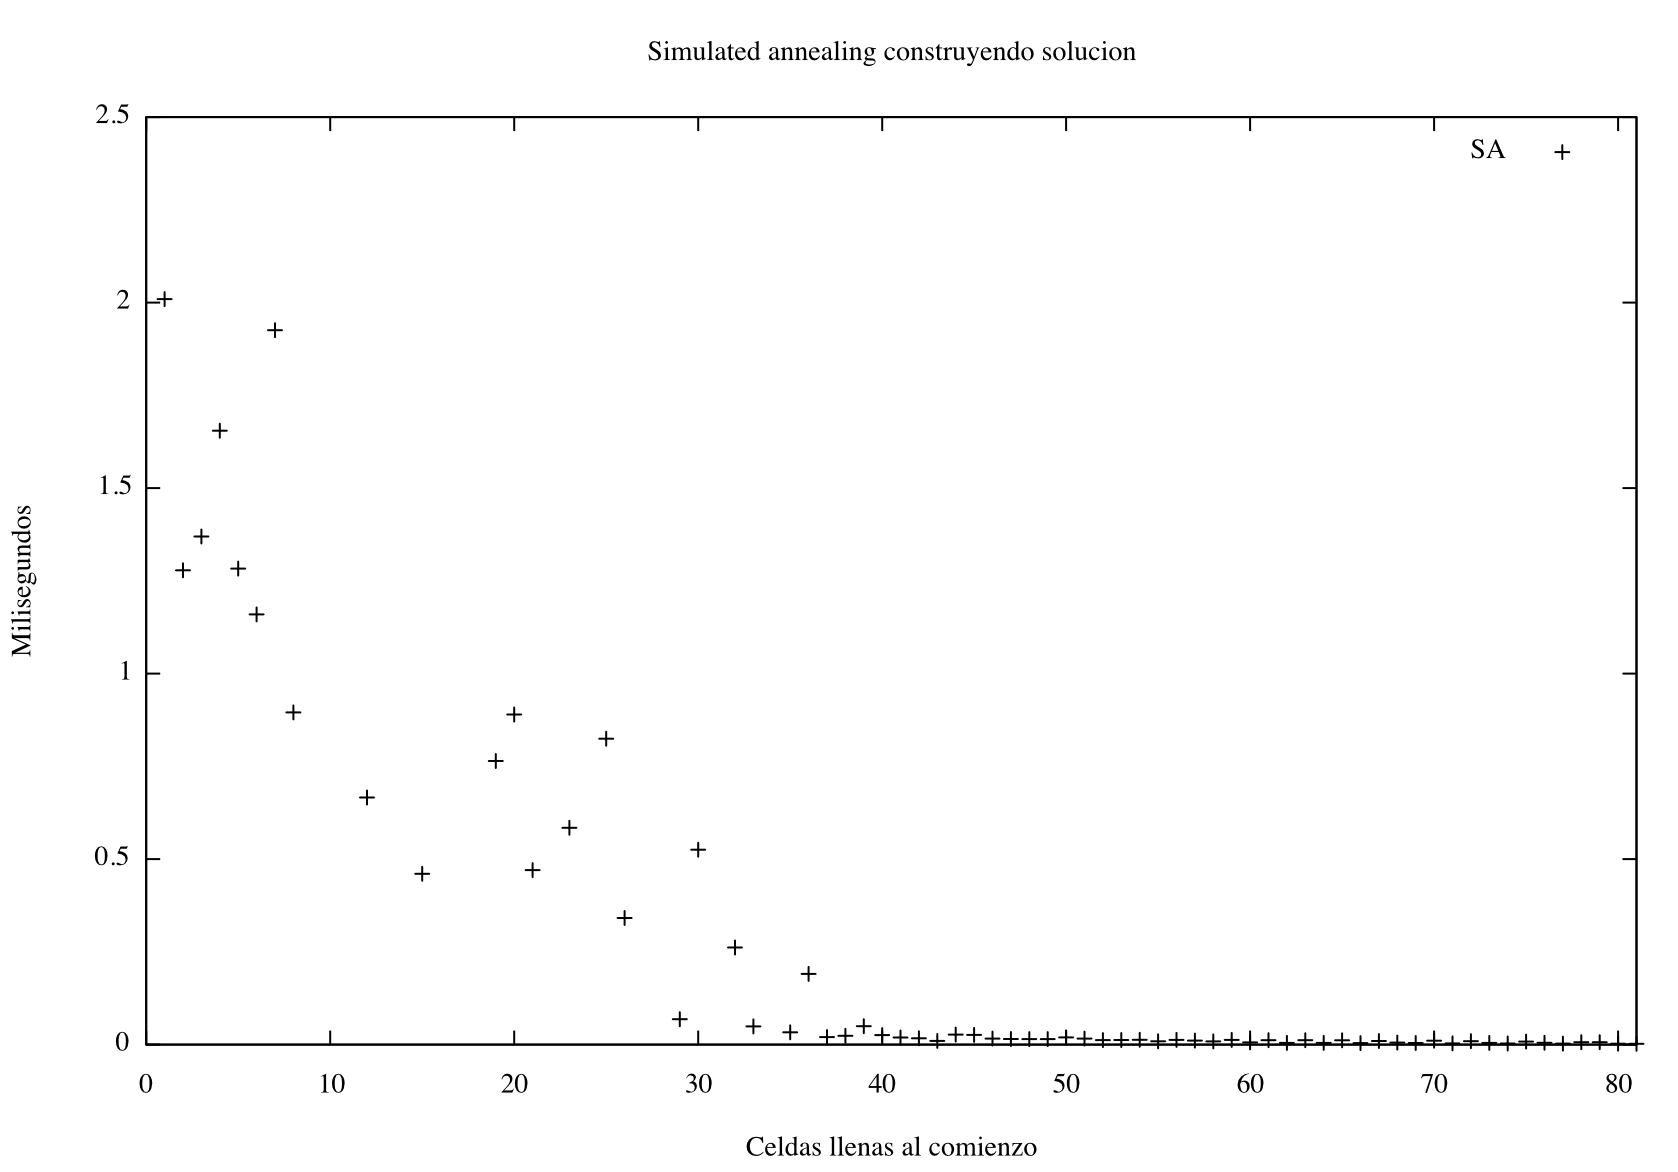
\includegraphics[scale=0.5]{imgs/randomSA.png}	\\
Clarmente se puede observar que a medida que el tablero esta mas lleno el tiempo es menor, eso es debido a la suma de varios factores, como que inicialmente infiere más celdas, son menos las vacias (que se convierte en menos iteraciones) y menos búsqueda de soluciones vecinas.\\\\

A continuación corrimos el algoritmo con 25 soluciones de diferentes niveles de dificultad, variando el factor de enfriamiento (o alfa):\\
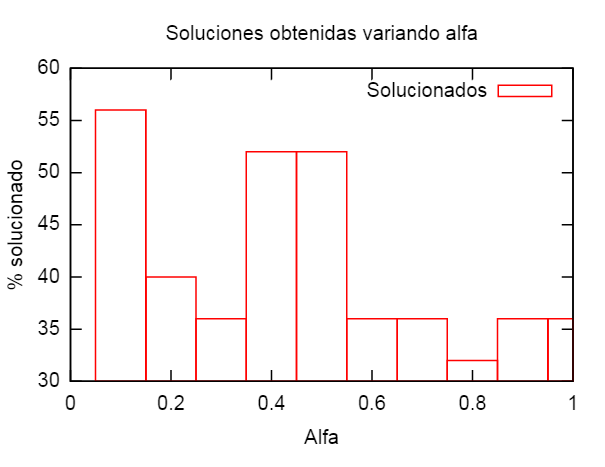
\includegraphics[scale=0.7]{imgs/porc_soluc.png}	\\
Si bien con valores intermedios (aprox 0.5) es donde se concentran las mejores soluciones, y que la mayor cantidad se logra con un 0.1, creemos en base a anteriores pruebas que el el factor de enfriamiento debería ser siempre mayor de 0.5 para que sea algo "lento" y no siempre elija ir por soluciones vecinas pero que tampoco las restrinja totalmente. 

\subsection{Hormigas}

Uno de los experimentos que realizamos es el tiempo de computo que demanda este algoritmo para finalizar, mas alla de sí efectivamente logra solucionarlo o no. Como mencionamos anteriormente utilizamos un probabilidad de 2 para el seguimiento de la feromona, en el siguiente experimento veremos el porque de esta eleccion.

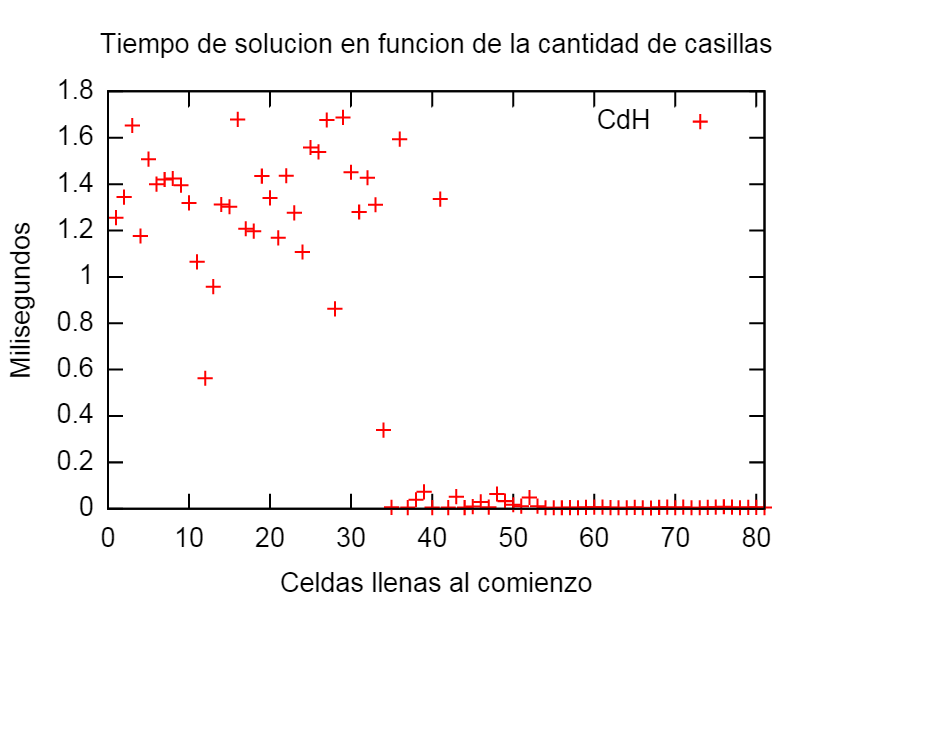
\includegraphics[scale=0.5]{imgs/resultados_random_hormigas.png}	\\
En este caso también podemos observar que a medida que el tablero esta mas lleno el tiempo es mucho menor. A partir de las 35 celdas blanqueadas aproximadamente vemos que el tiempo no es del todo regular, esto es porque hay casos en los que encuentra la solución rapidamente devido a su comportamiento random. Por otro lado los casos en los que no encuentra solución son los que mas demoran porque todas las hormigas intentan encontrarla, a diferencia de cuando se encuentra una solución ya que ahí frena la heurística y no siguen probando las demás hormigas.


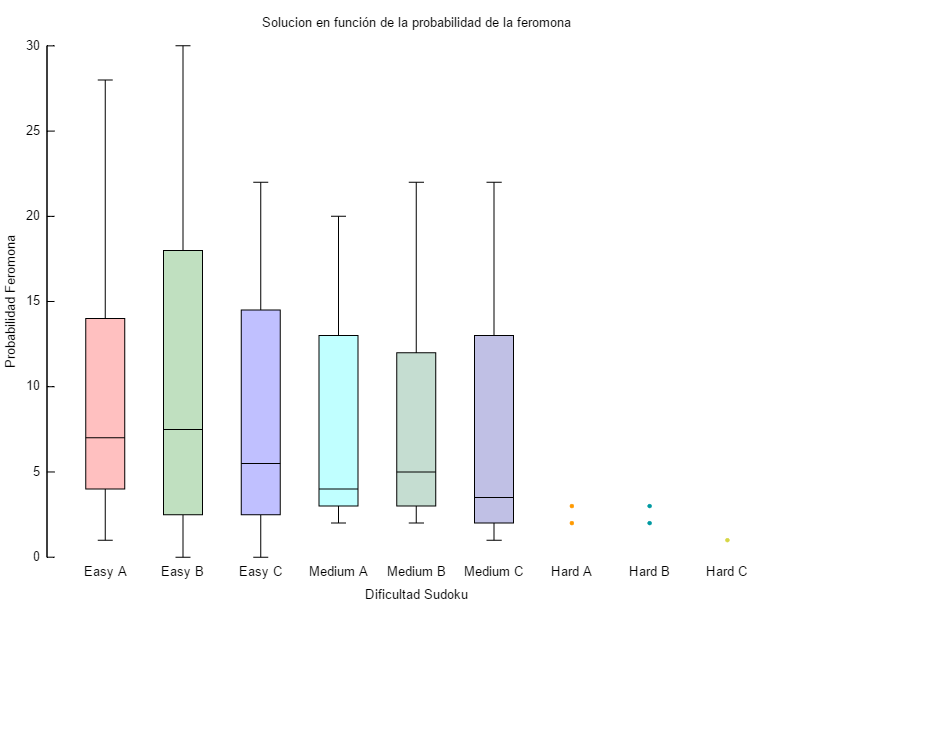
\includegraphics[scale=0.5]{imgs/solucion_hormigas_proba.png}
Otro experimento que nos pareció interesante fue el de contrastar diferentes niveles de dificultad de la configuración inicial de un Sudoku en base a si el algoritmo resuelve o no variando la probabilidad de la feromona. Y como resultado obtuvimos que para resolver la mayor cantidad de Sudokus conociendo la dificultad de antemano (preferentemente dificiles) la probabilidad tiene que estar en 2, ya que los casos dificiles estan en 2, pero si no importa la dificultad o no la sabemos, deberiamos incrementar ese número ya que, como se ve en el gráfico, los de dificultad facil/media utilizan una probabilidad de las feromonas mayor.
